%!TEX TS-program = xelatex
%!TEX root = ../../maxwell2018thesis.tex

\chapter[The Complex Searcher Model]{The Complex Searcher Model}\label{chap:csm}
In Part~\ref{part:intro}, we provided a comprehensive overview of the current state-of-the-art of user modelling within the field of~\gls{acr:iir} -- and stopping within search. In this chapter, we present an improvement on the current state-of-the-art, providing an outline of the main conceptual and theoretical contributions of this thesis, which include proposals of:

\vspace*{-2mm}
\begin{itemize}
    \item[\blueboxbold{(i)}]{a more complex and realistic user model -- the~\glsfirst{acr:csm} -- that captures the key interactions that take place during an~\gls{acr:iir} session (Section~\ref{sec:csm:csm}); and}
    \item[\blueboxbold{(ii)}]{an enumeration of a number of \emph{stopping strategies} that we will be evaluating (Section~\ref{sec:csm:stopping}).}
\end{itemize}
\vspace*{-2mm}

These outlines provide the foundations for the subsequent contributory chapters of this thesis that aim to both evaluate the quality of the proposed~\gls{acr:csm}, and the effectiveness of the proposed stopping strategies. Each of the stopping strategies that are proposed in this chapter are operationalised from a number of stopping heuristics defined in the literature, reviewed previously in Chapter~\ref{chap:stopping_background}. To complement the above, we also provide in this chapter \blueboxbold{(iii)} a high level description of the basic methodology we employ in subsequent chapters of this thesis (Section~\ref{sec:csm:methodology}).

\section{The Complex Searcher Model}\label{sec:csm:csm}
The~\glsfirst{acr:csm} is a high level, conceptual model of the search process that captures the key processes and decisions that are taken by a searcher during the information seeking process. Illustrated in Figure~\ref{fig:csm}, the~\gls{acr:csm} is an amalgamation and further development of prior, established models that capture the information seeking process. Discussed previously in Section~\ref{sec:stopping_background:models:conceptual}, prime examples of prior models include the Markov-based approach by~\cite{baskaya2013behavioural_factors}, and the searcher model proposed by~\cite{thomas2014modelling_behaviour}. These models (along with others) are in broad agreement with the general sequence of events that searchers undertake -- from issuing a query to examining documents for relevance. Refer to Figures~\ref{fig:baskaya_model_flow} and~\ref{fig:thomas_model} on pages~\pageref{fig:baskaya_model_flow} and~\pageref{fig:thomas_model} respectively for illustrations of the two aforementioned models.

Given the \emph{baseline models} outlined above and in Section~\ref{sec:stopping_background:models:conceptual}, the~\gls{acr:csm} offers a number of advancements in modelling the information seeking process. In this section, we outline:

\begin{itemize}
    \item{the \emph{flow} of the model, explaining the different steps and decisions that a searcher undertakes (Section~\ref{sec:csm:csm:flow});}
    \item{the different \emph{stopping decision points} of the model (Section~\ref{sec:csm:csm:stopping}); and}
    \item{the \emph{assumptions} that are made as part of the~\gls{acr:csm} (Section~\ref{sec:csm:csm:assumptions}).}
\end{itemize}

We begin however with an overview of the key advancements that the~\gls{acr:csm} provides over existing models of the information seeking process.

\begin{figure}[t!]
    \centering
    \resizebox{1\hsize}{!}{
    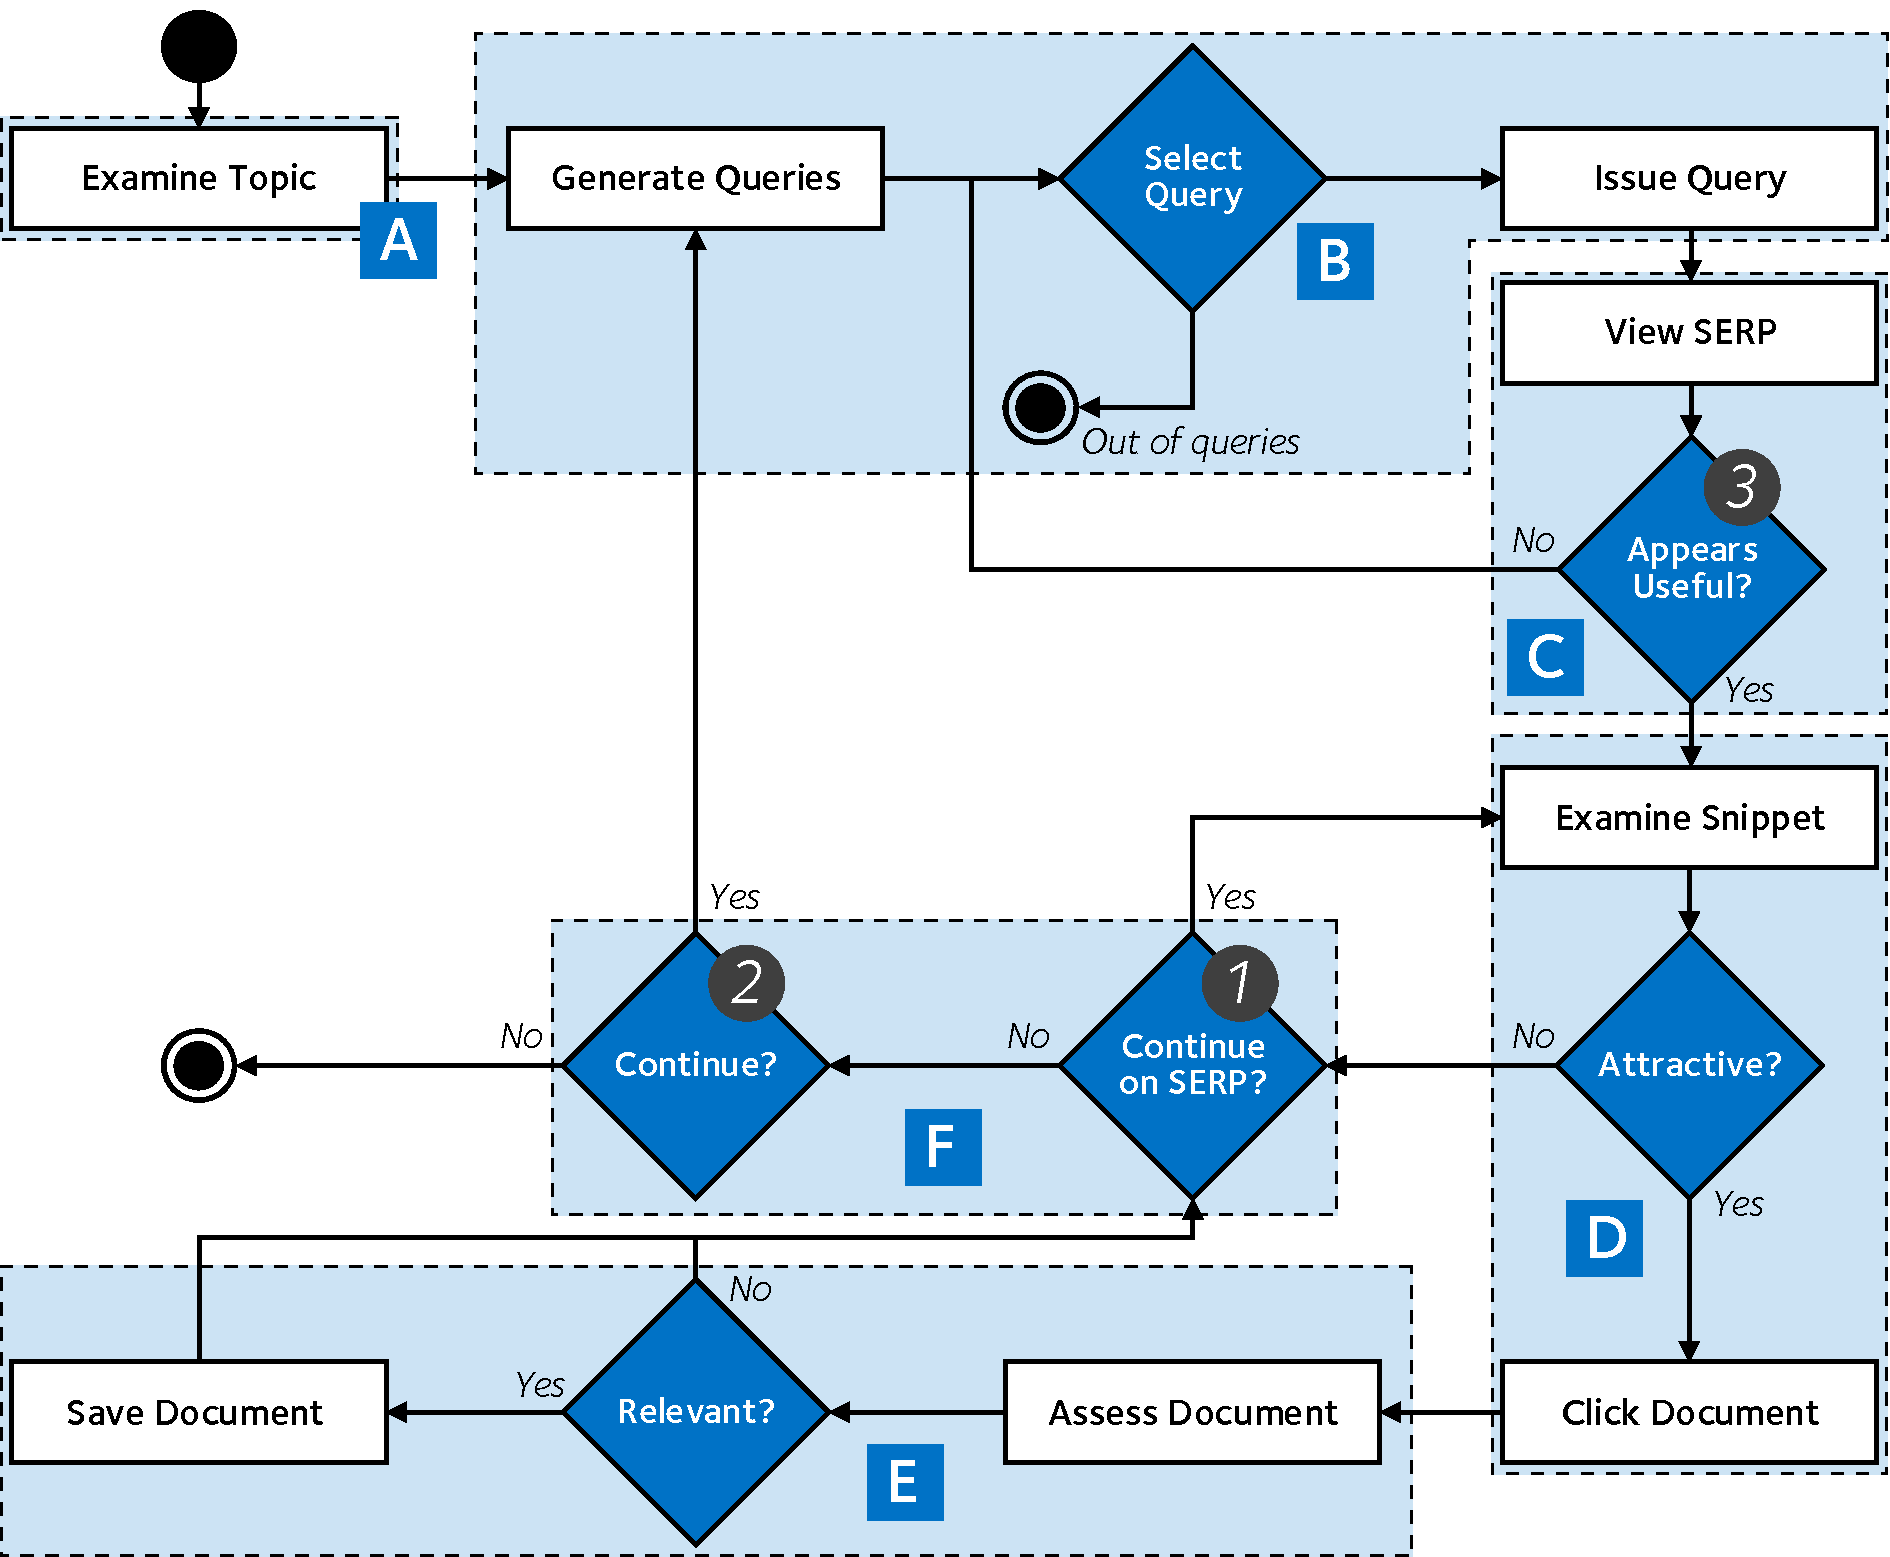
\includegraphics{figures/ch4-csm.pdf}}
    \caption[Flowchart of the~\glsfirst{acr:csm}]{A flowchart of the proposed~\glsfirst{acr:csm}, as used in experimental work discussed later in this thesis. Novel components that the work this thesis provides are highlighted by boxes \blueboxbold{A} and \blueboxbold{B}. The \emph{three} stopping decision points are highlighted with \blueboxbold{1}, \blueboxbold{2} and \blueboxbold{3} (refer to Section~\ref{sec:csm:stopping}). Refer to Section~\ref{sec:csm:csm:flow} for an in-depth explanation of the model.}
    \label{fig:csm}
\end{figure}

\subsection{Model Advancements}\label{sec:csm:csm:advancements}
The~\gls{acr:csm} provides two novel contributions to modelling the information seeking process. The contributions are highlighted as blocks \blueboxbold{A} and \blueboxbold{B} in the~\gls{acr:csm} flowchart provided in Figure~\ref{fig:csm}, and concerns:

\begin{itemize}
    \item[\blueboxbold{A}]{the advancement of modelling the \blueboxbold{querying} aspects of the searcher model; and}
    \item[\blueboxbold{B}]{the introduction of a \blueboxbold{third stopping decision} point concerning the \emph{overall impression} attained of a~\gls{acr:serp} by the searcher.}
\end{itemize}

In the remainder of this section, we discuss these two developments in more detail. While the querying advancements highlighted in block \blueboxbold{A} are novel and intuitive, they are not the core focus of this thesis -- the work detailed in block \blueboxbold{B} is of high relevance, and thus our discussion will be more in depth.

\subsubsection{Modelling the Querying Process}
\begin{publications_box}{Associated Publication}
Work on this advancement of the~\gls{acr:csm} can be found in the following publication.
\vspace*{-2mm}
\begin{itemize}
    \item{\bibentry{maxwell2016agents}}
\end{itemize}
\end{publications_box}

With a search session an inherently interactive process~\citep{ingwersen2005theturn}, a searcher is able to \emph{learn} and develop their mental model of the given information need as they examine information presented to them. As such, during a search task, a searcher may decide to reformulate their query as they obtain a better appreciation of the topic, and are able to formulate a better query, perhaps with descriptive key terms.

As such, the~\gls{acr:csm} provides the mechanism for a searcher subscribing to such a model to update the list of potential queries that could be issued once he or she has finished examining a set of results from the previous~\gls{acr:serp} (labelled as \blueboxbold{Generate Queries} in Figure~\ref{fig:csm}). This is in direct contrast to prior models of search, where queries were selected from a list generated at the start of the search session. This improvement in the modelling process permits a better representation of a searcher's so-called \emph{dynamic information needs}~\citep{borlund2003iir_model}.~\cite{maxwell2016agents} provides an in-depth discussion on this issue.

Once an updated list of queries has been generated, a searcher subscribing to the~\gls{acr:csm} will then make a decision as to \emph{what} query they should issue to the underlying search engine (labelled \blueboxbold{Select Query} in Figure~\ref{fig:csm}). Of course, at this point, a searcher may have exhausted all possible queries, and this is would therefore be a natural stopping point for the searcher. However, as previously discussed, we do not examine this particular component of the~\ref{fig:csm} in any great depth; we do however utilise \emph{querying strategies} that have been previously employed in the literature. Refer to \todo{Section~\ref{}} for more information on these strategies.


\subsubsection{\gls{acr:serp} Level Stopping}
\begin{publications_box}{Associated Publication}
Work on this advancement of the~\gls{acr:csm} can be found in the following publication.
\vspace*{-2mm}
\begin{itemize}
    \item{\bibentry{maxwell2018serp}}
\end{itemize}
\end{publications_box}

As previously mentioned in this section, the second major development, highlighted as block \blueboxbold{B} in Figure~\ref{fig:csm}, is the inclusion of an additional, third stopping decision point. This stopping decision point complements the two established stopping decision points, as discussed in Section~\ref{sec:stopping_background:models:conceptual:simple}.

As outlined by~\cite{maxwell2018serp}, this additional stopping decision point is motivated by the idea of the \emph{information scent} present on a given~\gls{acr:serp}. This was briefly discussed in Sections~\ref{sec:stopping_background:user_studies:understanding} and~\ref{sec:stopping_background:models:theoretical:ift}, and in these sections we highlighted the concept of \emph{proximal cues} providing insights into whether the presented page will yield information that will aid the searcher in satisfying their underlying information need. This has been previously demonstrated in prior studies~\citep{wu2014information_scent, ong2017scent_behaviour, maxwell2017snippets}. By operationalising the notion of information scent as the perceived performance of a given~\gls{acr:serp}, we argue that incorporating this additional activity and stopping decision point allows a searcher to obtain an \emph{impression} of the~\gls{acr:serp} before deciding to \emph{enter} the~\gls{acr:serp} and examine content in detail, or \emph{abandon} the~\gls{acr:serp} and move to the next activity. In other words, when a poor query is issued, the searcher will not expend effort examining content which will have a high probability of not being relevant to their information need. The notion of forming an impression is similar to the summary impressions formed by searchers subscribing to the model defined by~\cite{thomas2014modelling_behaviour}, as detailed in Section~\ref{sec:stopping_background:models:conceptual:simple}. However, in this model, the searcher does not form an overview of the~\gls{acr:serp}, but rather an impression of each summary. This allows him or her to then deduce whether it is enticing enough to examine in more detail.

This is analogous to the well-studied phenomenon of \emph{\gls{acr:serp} abandonment} in which limited interaction occurs with the searcher. This has been typically assumed to provide an indication of the searcher's \emph{dissatisfaction} with the presented results~\citep{dassarma2008serp_abandonment, chuklin2012serp_abandonment}. Thus, we provide, to the best of our knowledge, a model of the search process incorporating a path for a searcher to abandon a~\gls{acr:serp} that appears to be of poor quality (or a \emph{low scent}).

\subsection{Model Flow}\label{sec:csm:csm:flow}
With the underlying assumptions and developments of the~\gls{acr:csm} now outlined, we next provide a high-level description of the various stages of the model. The~\gls{acr:csm} is illustrated as a flowchart in Figure~\ref{fig:csm} on page~\pageref{fig:csm}. Here, the model is described, with an explanation of the different processes involved, and the associated stopping decision points.

When subscribing to the~\gls{acr:csm}, a searcher, once he or she has attained a form of information need, will begin by performing an \blueboxbold{examination of the topic}. This is typically considered to be provided by an experimenter in the form of a \emph{TREC topic}, where a searcher will be provided with a predefined \emph{topic description} of what will constitute as a relevant document (refer to Section~\ref{sec:csm:methodology:collection} for examples). The searcher will then begin to formulate an initial mental model of the topic, identifying key terms and phrases that could be potentially used to translate this information need into a query formulation~\citep{borlund2003iir_model}.

Once a model of the information need has been established, the searcher will then move onto the \blueboxbold{query generation}, \blueboxbold{query selection} and \blueboxbold{query issuance} stages. At this point, the searcher will employ some form of \emph{querying strategy} in order to formulate one or more queries from the underlying model of the information need, and then make a decision, \emph{selecting} one of the candidate queries to take forward and issue to the underlying search engine. As previously discussed, if all candidate queries have been exhausted, the searcher will then stop their search session at this point.

Once a query has been submitted the search engine, the searcher is then presented with the~\gls{acr:serp}. From here, the searcher is able to \blueboxbold{view the~\gls{acr:serp}} -- that is, obtain an \emph{initial impression} from examining the proximal cues presented to him or her. If the~\gls{acr:serp} does not appear to \emph{look good,} or offers a poor information scent, the searcher will abandon the~\gls{acr:serp} and proceed to then issue a further query from the list of candidate queries discussed previously.

If the~\gls{acr:serp} however appears to offer a high information scent, the searcher will then proceed to \blueboxbold{enter the~\gls{acr:serp}}. From here, individual \blueboxbold{snippets will be examined} in detail. As per the assumptions listed above, these are examined in a linear fashion. For each snippet, a judgement is made as to whether the searcher considers it to be sufficiently \blueboxbold{attractive} to click. If deemed sufficiently attractive, the link is clicked, and the searcher is then presented with the \blueboxbold{document} examined in full for an \blueboxbold{assessment}. Once complete, the searcher then makes a further decision with regards to the \blueboxbold{relevancy} of the document to the given information need (or topic, using~\gls{acr:trec} terminology). If deemed relevant, the document is then \blueboxbold{marked} as such, providing a simplistic means for determining what documents have been considered relevant and those that weren't -- refer to Section~\ref{sec:ir_background:user:evaluation:interactive_pr}.

Once the searcher has marked a document as relevant, he or she is returned to the~\gls{acr:serp}. At this point, the searcher must make a decision: \emph{should I continue to examine snippets on this current~\gls{acr:serp}?} This point is also reached by the searcher if he or she judges a snippet to have insufficient attractiveness to pursue further. If the answer is \emph{yes,} the next snippet is examined -- if the answer is \emph{no,} the searcher must then make a further decision. \emph{Given my overall search goals, have I met them? Should I continue my search session?} Search goals will vary between task type -- for ad-hoc retrieval, searchers will often attempt to find a predetermined number of relevant documents before a time limit expires. If the criteria have or criterion has not been met, the searcher will continue his or her search session by jumping back to the near start of the process, and undertake \blueboxbold{query generation} once more. If the stopping criteria have or criterion has been met, then the searcher will then abandon the search session, hopefully satisfied with what he or she has found.

Note that at each process -- whether it be issuing a query or examining a document for relevance -- a searcher will pay some form of \blueboxbold{cost} for the effort that they need to expend performing the aforementioned activity. All of the different components of the~\gls{acr:csm} -- whether they are activities or decision points -- can be instantiated in a number of different ways. For example, stopping strategies that we discuss below in Section~\ref{sec:csm:stopping} can be used to instantiate the different stopping decision points within the model. \todo{What about other bits?}

\subsection{Stopping Decision Points}\label{sec:csm:csm:stopping}
Of central focus to the work in this thesis are the \emph{stopping decision points} of the~\gls{acr:csm}. As previously discussed, the~\gls{acr:csm} contains an additional, third stopping decision point. This is in combination with the two established stopping decision points, as previously highlighted in Section~\ref{sec:stopping_background:models:conceptual:simple} on page~\pageref{sec:stopping_background:models:conceptual:simple}.

The three stopping decision points that the~\gls{acr:csm} considers are listed below. While these are explained in Section~\ref{sec:csm:csm:flow}, it is nevertheless good practice to enumerate them.

\begin{itemize}
    
    \item{\blueboxbold{\gls{acr:serp} Level Stopping} considers the point at which a searcher can abandon a~\gls{acr:serp} after attaining an \emph{initial impression} of the presented~\gls{acr:serp}, thus saving a searcher from examining summaries in depth if the~\gls{acr:serp} appears to be of poor quality.}
    
    \item{\blueboxbold{Snippet Level Stopping} As previously mentioned, this is sometimes labelled as \emph{query level stopping} in the literature. We name this decision point snippet level stopping to remove any ambiguity between~\gls{acr:serp} level stopping and this point. Snippet level stopping considers the depth to which a searcher will traverse a list of results, before deciding to stop their examination.}
    
    \item{\blueboxbold{Session Level Stopping} Finally, session level stopping concerns the notion of when a searcher will decide to terminate their search session altogether. This could be constrained by time limits, or some predetermined notion of how many relevant items they have found.}
    
\end{itemize}

Figure~\ref{fig:csm} on page~\pageref{fig:csm} also provides a visual illustration of the stopping decision points within the wider~\gls{acr:csm} flowchart. Decision points \blueboxbold{1}, \blueboxbold{2} and \blueboxbold{3} represent snippet level stopping, session level stopping and~\gls{acr:serp} level stopping respectively.

How these stopping decision points are operationalised is dependent upon a variety of different factors. For example, the task type is highly likely to influence the overall session stopping strategy that is employed. The literature, as overviewed in Section~\ref{sec:stopping_background:heuristics} provides a number of heuristics to potentially operationalise stopping. These are primarily geared towards the concept of snippet level stopping.

\subsection{Clarifications and Assumptions}\label{sec:csm:csm:assumptions}
As with any model of a real-world phenomenon, the~\gls{acr:csm} also makes a number of key assumptions. Along with clarifications of the model, we list and detail these assumptions below.

\noindent
\blueboxbold{Considering Ad-Hoc Retrieval} The~\gls{acr:csm} considers \emph{ad-hoc retrieval,} a type of search task previously discussed earlier in Section~\ref{sec:ir_background:basics:cranfield:trec}.\footnote{This clarification is included at the request of Distinguished Professor Nicholas Belkin (Rutgers University, NJ, USA), who discussed that the task type the~\gls{acr:csm} models should be clearly defined. This was done at the first \emph{ACM CHIIR} Doctoral Consortium in Chapel Hill, NC, USA -- refer to~\cite{maxwell2016dc} for the associated publication.} Of course, many other different types of search task exist, such as, for example, navigational and patent searching. Ad-hoc retrieval is foundational to many areas of~\gls{acr:ir}\footnote{Referring to \emph{Microsoft} Senior Applied Scientist Peter Bailey's \emph{SIGIR} paper writing tips (available at~\url{https://www.microsoft.com/en-us/research/people/pbailey/} -- last accessed May 1\textsuperscript{st}, 2018), \emph{``there is more to life than ad-hoc''} (tip 10). We agree with this statement, but also argue in the main narrative that the similarities between ad-hoc and other search tasks are similar in nature, making it a sensible choice to consider.} -- but the similarities between ad-hoc and other types of search task provide motivation for selecting such a task to model.

Take, for example, a navigational task. A searcher, wishing to find the electronic commerce site \emph{Amazon}, may issue a query to a commercial web search engine. The query, \texttt{amazon}, yields a series of results presented to him or her on a~\gls{acr:serp}. Typically, if the intent is correctly understood by the search engine, the first result in the verticals links the searcher to Amazon, satisfying his or her information need. This process is largely the same of the~\gls{acr:csm}, as illustrated in Figure~\ref{fig:csm}. Unlike the~\gls{acr:csm} however, the searcher will not complete later stages of the model, such as marking the identified document as relevant -- the searcher will simply abandon the search session.

The argument for using ad-hoc retrieval as the underpinning of the~\gls{acr:csm} is therefore simple. By modelling ad-hoc retrieval, this essentially guarantees that the entire search process -- from query formulation to identifying relevant documents -- is repeated a number of times. As we are modelling the search process in its entirety -- not individual components in isolation -- this makes ad-hoc retrieval a sensible choice.

\noindent
\blueboxbold{Choosing a Search Engine} A searcher, when subscribing to the~\gls{acr:csm}, is assumed to have already undertaken the necessary steps in selecting the search engine most likely to satisfy his or her information need. This is important to clarify, as certain models of information seeking proposed in the literature -- such as the model proposed by~\cite{thomas2014modelling_behaviour} -- include the notion of selecting a search engine within the wider information seeking model. Of course, this is an important step -- selecting a patent search engine\footnote{As opposed to general purpose, commercial web search engines such as \emph{Google} or \emph{Bing,} agencies such as the European Patent Office provide bespoke patent search engines -- refer to \url{https://worldwide.espacenet.com/} for an example (last accessed May 1\textsuperscript{st}, 2018).} for a patent search task would be a prudent choice. We however consider this step superfluous to the requirements of the~\gls{acr:csm} -- the model purely considers the interactions between the user and the search engine, not decisions made before or after.

\noindent
\blueboxbold{Bad and Good~\gls{acr:serp} Abandonment} When considering whether the~\gls{acr:serp} should be abandoned (via the new stopping decision point, summarised in Section~\ref{sec:csm:csm:stopping}), we assume that this is under the pretence of \blueboxbold{bad abandonment} (i.e. a dissatisfaction of the presented results). This is in contrast to the notion of \emph{good abandonment}~\citep{khabsa2016good_abandonment}, which we do not consider in the presented~\gls{acr:csm}. However, future refinement of the model may lead to the ability for the~\gls{acr:csm} to discern between the two -- refer to Figure~\ref{fig:csm_bad_good} for a potential solution to this issue. Indeed, this may be more applicable in future research -- good abandonment is typically prevalent in contemporary~\gls{acr:ir} research (especially on small-screen devices such as smartphones). Furthermore, with the addition of contemporary~\gls{acr:serp} components such as the information card~\citep{bota2016information_cards}, certain information needs can be satisfied by examining the~\gls{acr:serp} without needing to click on any results.

\begin{figure}[t!]
    \centering
    \resizebox{1\hsize}{!}{
    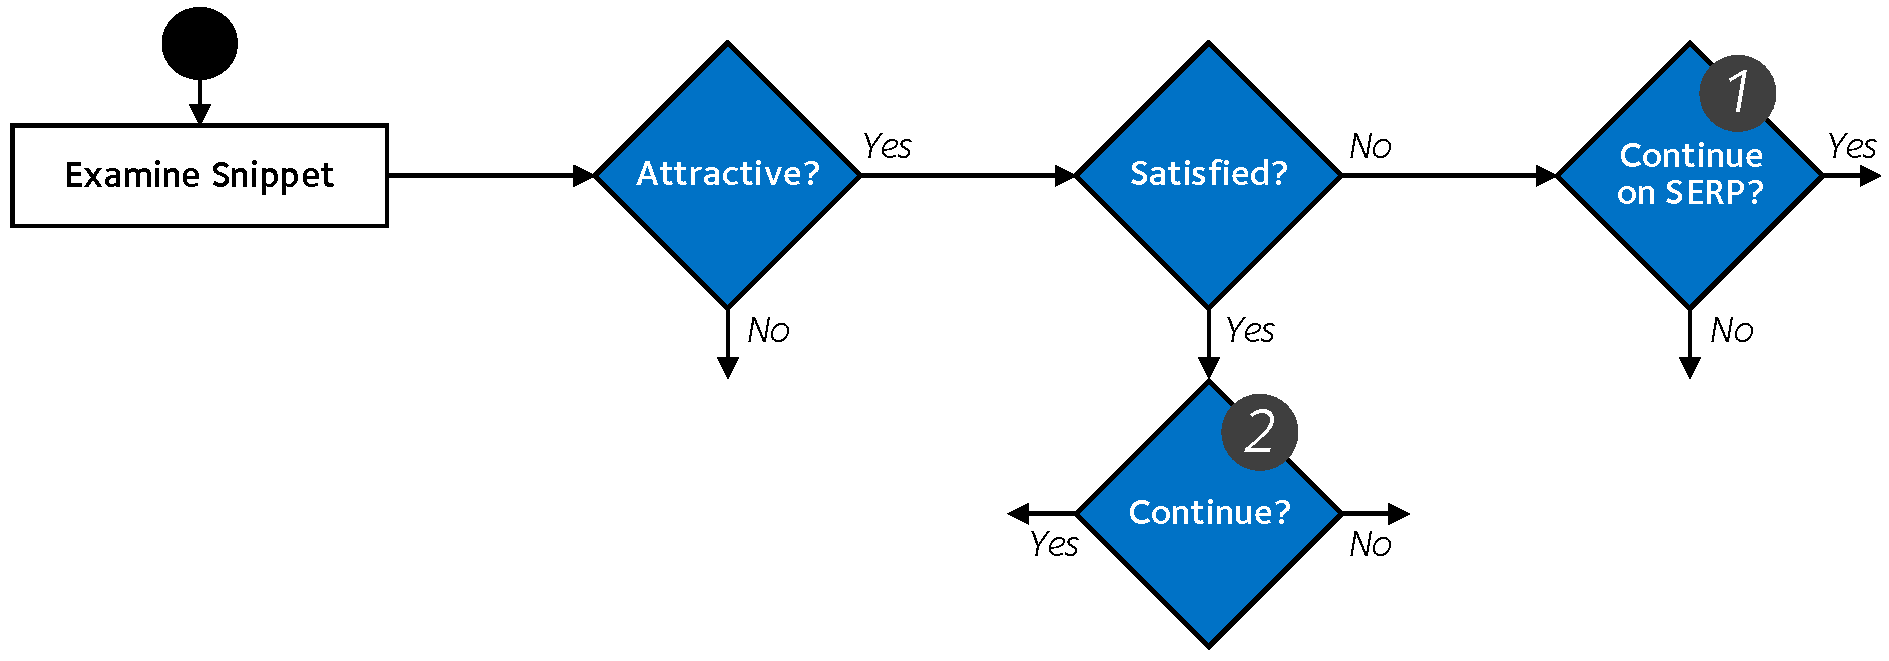
\includegraphics{figures/ch4-good.pdf}}
    \caption[Flowchart considering good abandonment]{A potential solution to also considering good abandonment. After examining a snippet for attractiveness, an additional decision point could allow a searcher to determine that examining the snippet itself satisfies their information need, and thus provide a means by which the searcher could then stop examining results, or stop their search session altogether.}
    \label{fig:csm_bad_good}
\end{figure}

\noindent
\blueboxbold{Simple~\glsplural{acr:serp}} When considering the~\gls{acr:serp} presented to a searcher as a whole, we make three simplifying assumptions within the~\gls{acr:csm}. These are listed and detailed below.

\begin{itemize}
    \item{\blueboxbold{Ten Blue Links} Under the~\gls{acr:csm}, a~\gls{acr:serp} will consist only of one set of \emph{verticals,} i.e. the traditional \emph{ten blue links} that are still present in contemporary~\glsplural{acr:serp}. Of course, we acknowledge that additional components are present in contemporary~\glsplural{acr:serp}, such as multimedia content in federated search~\citep{chen2012federated_search_click_model}.}
    \item{\blueboxbold{Linear Examination Order} Once a searcher has decided to examine a~\gls{acr:serp} in detail, the result summaries presented to the searcher will be examined in the order in which they appear. There is evidence to suggest that real-world searchers examine results from top to bottom, as demonstrated by~\cite{joachims2002click_model} and~\cite{joachims2005click_model}, for example. Click models, such as the \emph{cascade model}~\citep{craswell2008click_models}, have been developed that employ this assumption. Such approaches are subject to \emph{position bias,} where the searcher trusts the results of the retrieval algorithm, assuming that the first result presented in the verticals is the most relevant to their information need.}
    \item{\blueboxbold{No Pagination} The~\gls{acr:csm} also assumes that the~\gls{acr:serp} presented to a searcher is of a single page, and no pagination of results exists. This does simplify the modelling process somewhat, with pagination not considered in prior information seeking models that consider the search session as a whole.}
\end{itemize}

\subsection{Stochastic and Deterministic}
\begin{publications_box}{Associated Publication}
Work discussing the notion of incorporating state and agency into the~\gls{acr:csm} can be found in the following publication.
\vspace*{-2mm}
\begin{itemize}
    \item{\bibentry{maxwell2016agents}}
\end{itemize}
\end{publications_box}

In this section, should I explain the difference between stochastic models of search, and deterministic models of search?
So, in a previous section, we detailed different approaches to simulation.

Stochastic considers a `roll of the dice' to determine whether a searcher will click on a link, for example $P(C)$. And that can be drilled down even more, to consider probability of a click given that it is relevant to some gold standard $P(C|R)$.

Other alternative is to instantiate the model using deterministic components.
So that the searcher is able to deduce, without grounding, what is relevant and not. Dependent upon various components like language models, and is much more complex. This is more in tune with attempting to model the cognitive functions going on inside someone's brain, and is not really the focus of this thesis.

However, we have explored this in detail. In~\cite{maxwell2016agents}, we looked at the notion of developing intelligent search agents with the~\gls{acr:csm}. (Short explanation of paper).

These are dependent upon the state of a user. We argue that even a simple implementation of the CSM itself has some form of state, because it needs to remember things like: what documents it has clicked on, what documents it has marked, and so forth. It needs to keep track of queries it has issued, so it does not issue duplicates. Basic things. In this agency paper, we took it further, so the searcher was able to `learn' and make informed decisions (i.e. training a language model) at each iteration of the search process.

So... in this thesis, we consider only stochastic models of search, where the simulations are grounded with some prior probabilities extracted from interaction data. The approach is discussed more in Section~\ref{sec:csm:methodology}.